\section*{Dioptra}

\item 
\begin{enumerate}
	\item (*) Demostrar que un haz homocéntrico de pequeña abertura que incide casi normal sobre una dioptra plana, da lugar a otro haz homocéntrico.
	Considere los casos de objetos reales y virtuales.
	\item Una moneda se encuentra en el fondo de un vaso que contiene agua hasta una altura de 5 cm ($n_{agua}=1.33$).
	Un observador la mira desde arriba, ¿a qué profundidad la ve?
	\item (*) Estimar la máxima abertura de un haz homocéntrico, para que la posición de la imagen, formada por una única superficie plana, quede determinada con un error del 2\%. 
\end{enumerate}


\item (*) Usando los resultados del problema anterior demuestre que un haz homocéntrico de pequeña abertura, al atravesar una lámina de caras paralelas, da lugar, en primera aproximación, a otro haz homocéntrico.
Halle la posición de las sucesivas imágenes. 


\item
\begin{minipage}[t][1.4cm]{0.52\textwidth}
	Analice la figura con la ley de Ibn Sahl - Snell haciendo uso de la aproximación paraxial $\alpha \approx \sen( \alpha ) \approx \tan( \alpha )$ (lo mismo pasa con $\beta$ y $\varphi$) 
\end{minipage}
\begin{minipage}[c][0.4cm][t]{0.4\textwidth}
	\begin{tikzpicture}
	\def \arcoDioptra{30};
	\def \radioDioptra{3};
	\coordinate (origenDioptra) at (-1,0);
	\coordinate (so) at (-2,0);
	\coordinate (centroDioptra) at (\radioDioptra,0);
	\coordinate (si) at (5,0);
	\coordinate (interseccionDioptra) at ({2 - \radioDioptra*cos(25)},{\radioDioptra*sin(25)});
	\draw [thin, dashed] (-2.5,0) -- (5.5,0);% node [midway, anchor=north] {eje óptico} ;
	\draw [ultra thick] (origenDioptra) arc(180 : 180 - \arcoDioptra : \radioDioptra);
	\draw [ultra thick] (origenDioptra) arc(180 : 180 + \arcoDioptra : \radioDioptra);
	\draw [thin, -LaTeX] (centroDioptra) -- (interseccionDioptra) node [midway, below, rotate = -18] {\(R\)};
	\draw [-latex] ($(centroDioptra) - (1,0)$) arc(180 : {180-atan{0.34}} : 1) node [midway, left] {$\beta$};
	\draw [thick, blue, -LaTeX] (so) -- (interseccionDioptra);
	\draw [-latex] ($(so) + (0.6,0)$) arc(0 : {atan{0.57}} : 1) node [midway, right] {$\alpha$};
	% \dimline[line style ={line width=0.7}]{($(so) - (0,0.5)$)}{($(origenDioptra) - (0,0.5)$)}{$s$};
	\dimline[line style ={line width=0.7},extension start length=-0.5,extension end length=-0.1]{($(so) - (0,0.5)$)}{($(origenDioptra) - (0,0.5)$)}{$s$};
	\draw [thick, blue, LaTeX- ] (si) -- (interseccionDioptra);
	\draw [-latex] ($(si) - (1.7,0)$) arc(180 : {180-atan{0.4}} : 1) node [midway, left] {$\varphi$};
	% \dimline[line style ={line width=0.7}]{($(origenDioptra) - (0,0.5)$)}{($(si) - (0,0.5)$)}{$s'$};
	\dimline[line style ={line width=0.7},extension start length=-0.1,extension end length=-0.09]{($(origenDioptra) - (0,0.5)$)}{($(si) - (0,0.5)$)}{$s'$};
\end{tikzpicture}

	% 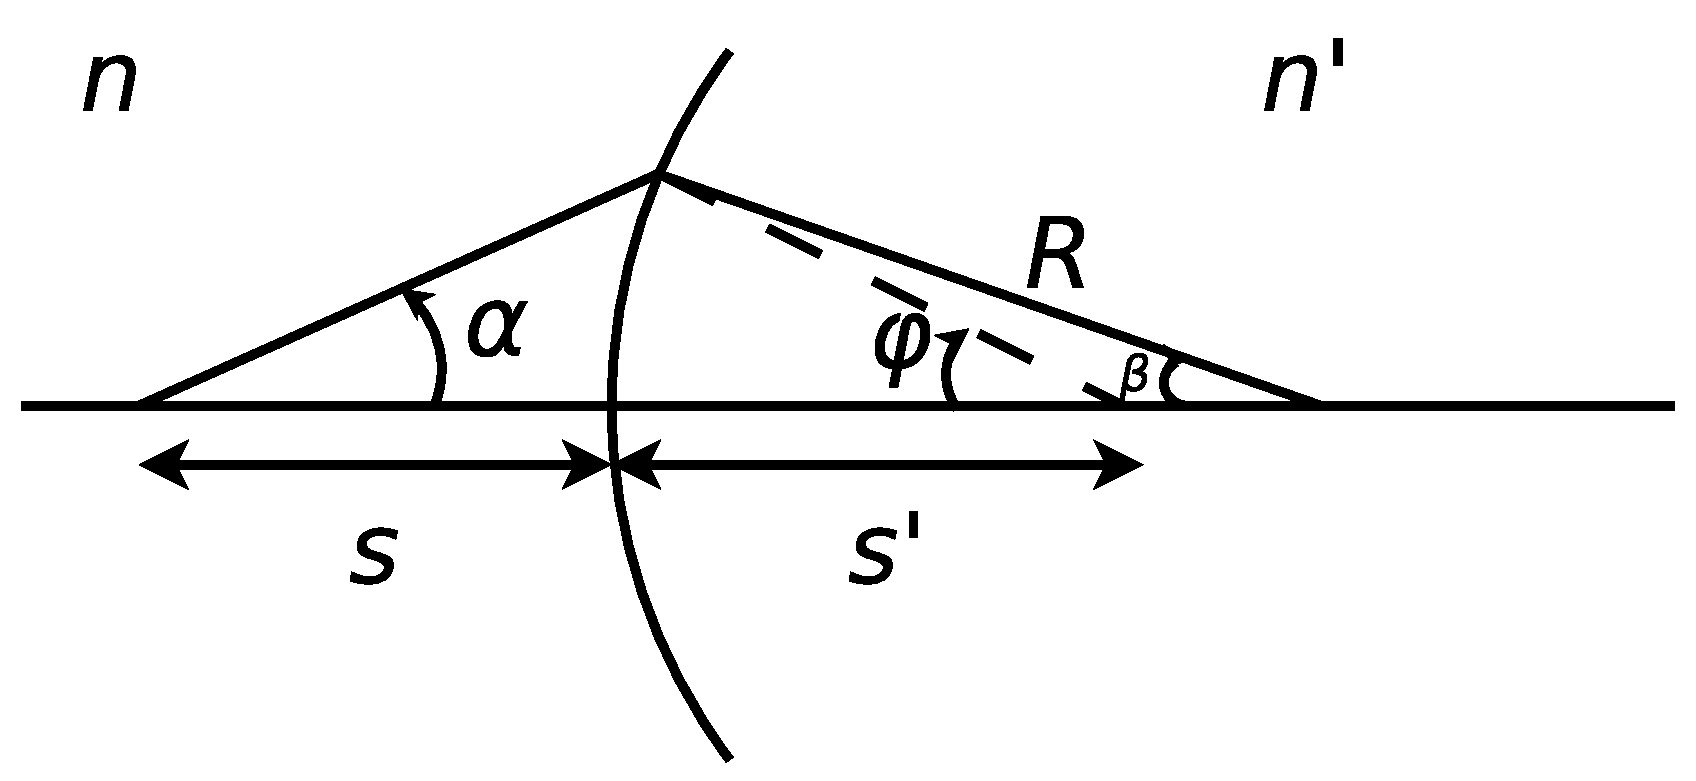
\includegraphics[width=\textwidth]{ej3-15}
\end{minipage}
\begin{enumerate}
	\item
	Obtenga la ecuación de las dioptras esféricas
	\[
		\frac{n'}{s'}\mp\frac{n}{s}=\frac{(n'-n)}{R} .
	\]
	Discuta el doble signo, asociándolo con la convención de signos que se utilice.
	\item ¿Cuándo una dioptra esférica es covergente/divergente? 
	Realice los gráficos de $s'$ vs. $s$ para ambos casos.
	Analice a partir de los mismos para qué posiciones de los objetos son reales o virtuales las imágenes, si son directas o invertidas, y lo mismo para objetos virtuales.
	\item ¿Pueden ser iguales las dos distancias focales de una dioptra?
	Justifique su respuesta.
\end{enumerate}
